% Chapter 3

\newcommand\tab[1][1cm]{\hspace*{#1}}
\newcommand\Doubletab[1][2cm]{\hspace*{#1}}

\chapter{Elements of Reinforcement Learning} 
\label{Chapter3} % For referencing the chapter elsewhere, use \ref{Chapter3}



In this section, we introduce the basic theoretical concept of reinforcement learning and the mathematical preliminaries associated with it.
In particular, we start from the formalism of MDP and then see as an example one of the first simple approaches to resolution.
For further details, refer to chapter 3,4,5,6 of Reinforcement Learning: An Introduction
\cite{bib:2018Sutton_RLBook}


\section{Markov Decision Process}
In the Reinforcement Learning context, there is an agent that learns how to achieve its goal directly by interaction with the environment. 

\textbf{Markov Decision Processes} formally describe both the environment and the agent. To understand the MDP is necessary to introduce some concepts like \textit{Stochastic Variable}, \textit{Stochastic Process}, \textit{Markov Chain}.

\subsection{Markov Chain}
We start introducing the Stochastic Variable and Stochastic Process.

\textbf{Stochastic Variable}: is a variable, usually expressed with a capital letter, whose possible values depend on a particular outcome of a random phenomenon. 
They are also known as Random Variables and, they can be \textit{Discrete} or\textit{Continuous}.
\\

\textbf{Stochastic Process}: is a collection of discrete stochastic variables each one indexed by a value that represents a step of time in the process.
This index is usually expressed like time step t.
\\

So in a particular time step t, the process is in one of all its possible states mathematically expressed by a stochastic variable.
More formally $s_t \in S$ where $S = \left\{ s_0,s_1, ... , s_m \right\} $.
The set of all possible states is called \textbf{State Space}.

The evolution of the system during the time is represented by a progression of the index from the current variable $s_t$ to the next one $s_{t+1}$.

The rule by which the index progress is called  \textbf{Transition Function}, and it is not deterministic, so the process produces different sequences of states each time it is run, even if it always starts from the same initial state.
The value of a variable can influence that of the variables that follow it. 
Therefore the progression of the states depends on the whole sequence starting from the initial state.
More formally this rule is expressed with a probability distribution: $$ P[S_{t+1} | S_1, ..., S_t] $$



A \textbf{Markov Chain} is a particular case of stochastic process that respects the Markov Property: "The future is independent of the past given the present".

This means that each state must capture all the relevant information from the environment at that moment, so when you have the state, you could throw away all the history.
In other words, thanks to the Markov Assumption the transition function is conditionally independent from the past state if the current state are given.

More formally we say:
\begin{equation*}
    P[S_{t+1} | S_t] = P[S_{t+1} | S_1, ..., S_t] 
\end{equation*}    


\subsection{Markov Decision Process}
A Markov Decision Process (MDP) is an extension of the \textit{Markov Chain} that includes an agent that performs actions in the process, that in this context is called \textbf{Environment}.


The agent influences the evolution of the environment with its actions.
So the state transition probability change including also the actions: $P(s, a, s^{'}) = [S_{t+1} = s' | S_t = s, A_t = a] $.
The purpose of the agent is to led the evolution of the environment to a particular set of states, called \textbf{Goal States}.
At every time step, the agent makes a decision on which is the best action to take.
The process by which the agent chooses an action from the given state is represented by with a function, called \textbf{Policy Function}.
It is represented by a probability distribution associated with every state in input. 
More formally we say: an agent follows the policy $\pi$ for every time step $t$ and for each $s_t \in \mathcal{S}$ it executes the action $a_t \in \mathcal{A}$ according to the probability $\pi(a|s)$.
To guide the agent's decision process we assign a reward signal (a real number $r_t\in 	\mathbb{R}$) to every action that it executes. 
Having this reward signal we can say if a state is more desirable then one other.



\begin{figure}[h]
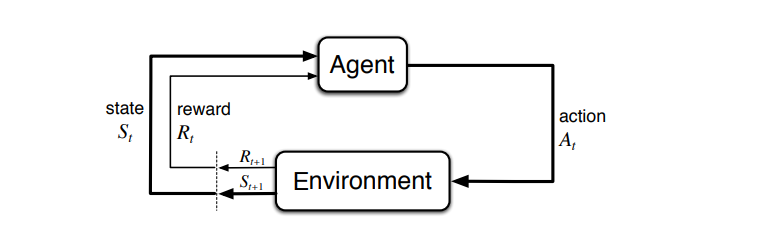
\includegraphics[width=\textwidth]{pictures/mdp_schema}
\caption{The agent-environment interaction in a Markov decision process. (Image source: Sec. 3.1 Sutton and Barto (2017) \cite{bib:2018Sutton_RLBook}}
\centering
\end{figure}


The agent receives the initial state of the environment and uses it to choose an action. 
Then, the environment evolves its state into a new one depending on both the current state and the agent's action. 
At this point, the agent receives two inputs: the new state and the reward signal.
It uses the reward signal to improve its own decision method and the new state to choose the next action.

This process is repeated iteratively until a final state is reached.

Every step of this process is called \textbf{Transition}: ${s_t,a_t,r_t,s_{t+1}}$.
The list of all transition from initial state to the final one is called \textbf{Episode}.

There are some particular classes of MDP that are called \textbf{Infinite MDP} in which do not exist a final state, but the construction of the reward function is still possible.

The agent can use the reward signal to know what is a good move and what it isn't.
With this knowledge, it can learn the best strategies to achieve its goal.
Assuming to be in a particular time step t of a finite MDP the definition of cumulative reward, from step t to the final step T, is:

\begin{equation*}
G_t = R_{t} + R_{t+1} + R_{t+2} + ... + R_{t+T}  
\end{equation*}
So the objective of the reinforcement learning is to find the parameters $\theta^*$  to the policy function $\pi^*$ that maximizes the expected cumulative reward of all the episodes.
\begin{equation*}
\label{policy_function}
    \pi^* = argmax_\theta E_{\tau \sim \pi_\theta} \left [\sum_{t}^{T}    r(s_t, a_t)  \right ]
\end{equation*}

The reward value is often presented with the \textbf{Discount Factor}, generally expressed with the symbol $\gamma \in [0,1]$. 
The purpose of the discount factor is to define the priority that the agent assigns to the future expected reward with respect to the immediate ones.
So the formula of the discounted expected cumulative reward becomes:

\begin{equation*}
G_t = R_{t} + \gamma R_{t+1} + \gamma^2 R_{t+2} + ... = \sum_{k=0}^\infty \gamma^k R_{t+k} 
\end{equation*}


Notice that the lower the gamma factor is and the more the agent will prefer the immediate reward than the long term values. 

This value not only helps to represent the uncertainty about the future but it is also mathematically convenient because it can be used to end up with a finite number also in case of infinite sequence of states (using the sum of infinite series) if $\gamma < 1$. 
So it can be very useful for Infinite MDP. 





To conclude a MDP is a tuple defined by $<\mathcal{S},\mathcal{A},\mathcal{P},\mathcal{R}, \mathcal{Z}, \gamma>$:
\begin{itemize}
  \item a finite set of states $\mathcal{S}$ 
  \item an initial state $s_0$
  \item a finite set of actions $\mathcal{A}$
  \item a state transition probability $P(s, a, s^{'}) = [S_{t+1} = s' | S_t = s, A_t = a] $
  \item $\mathcal{R}$ is a reward function, $\mathcal{R}(s,a)$ 
  \item $\gamma$ is a discount factor $ \gamma \in [0,1].$
\end{itemize}



\subsection{Partially Observable Markov Decision Process}
A Partially Observable Markov Decision Process, also called POMDP, is a particular case of MDP in which the agent hasn't direct access to the full states but for each time step,it makes an observation that depends on it. 

A POMDP in defined by a tuple $<\mathcal{S},\mathcal{A},\mathcal{P},\mathcal{R},\mathcal{Z},\gamma>$, so respect to the classic MDP it required also:
% \mathbb{R} set of real numbers
\begin{itemize}
  \item a finite set of observations O
  \item an observation function, $\mathcal{Z}(o,a,s^{'}) = P\left [O_{t+1} = o | S_{t+1} = s^{'}, A_t = a \right]$
  
\end{itemize}

In POMDP the transition is composed by the action, the reward and the observation of the environment. 
We define the entire sequence, from initial state to some time step t, as history $H_t$:

\begin{equation*}
    H_t = O_0, A_0, R_0, O_1, \dots, O_{t-1}, A_{t-1}, R_{t-1}, O_{t}
\end{equation*}

During the history, the agent formulates hypothesis on what is the effective state behind each observation. To build this hypothesis, that is called \textit{belief state}, it uses the history.

So, more formally, a belief state b(h) is a probability distribution over states, conditioned on the history h:

\begin{equation*}
b(h) = \left (P\left[ S_t = s^{1} | H_t = h \right] , ... , P\left[ S_t = s^{n} | H_t = h \right]\right) 
\end{equation*}
With the belief state the Markovian Assumption is no more valid.

\section{Solving Markov Decision Process}
In this section we introduce the two principal approach to solve an MDP, that are called \emph{prediction problem}, used when a fixed policy is given and \emph{control problem} used when there are no policy available. 

\subsection{Prediction Problem}
The prediction problem consist of evaluating a given policy function in an unknown MDP.
The metric used to evaluate a policy is the \textbf{value function}.

For every state the value function estimates how good it is for the agent that follows its given policy in the environment.
This value is a scalar number and it is expressed in terms of the expected cumulative discounted reward from the given state to the end.  
So, more formally:
\begin{equation*}
v_\pi(s) = E_\pi \left[ G_t | S_t = s \right]. 
\end{equation*}

To explain how it works we first need to define a partial ordering over policies. 
One policy is better than another when it produces a greater value for each state. 
More formally: 
\begin{equation*}
\pi \geqslant \pi^{'} \forall s \in \mathcal{S} \iff v_\pi(s)  \geqslant  v_\pi'(s) \, \forall s \in \mathcal{S}
\end{equation*}
So also the definition of the best policy is related to the value function:
\begin{equation*}
\pi_* \geqslant \pi \, \forall \pi \, (\forall s \in S) \iff v_*(s)  \geqslant  v_\pi(s)\, \forall s \in \mathcal{S}
\end{equation*}

From Sutton's book \cite{bib:2018Sutton_RLBook}, in chapter 3.6, we can read: "there is always at least one policy that is better than or equal to all the other policies. This is an \textbf{optimal policy}." 
Starting from the definition of the value function, it is possible to derive the iterative formulation for any arbitrary state.

\begin{align}
    v_\pi(s) &= E_\pi \left [ G_t | S_t = s \right ] \\
    v_\pi(s) &= E_\pi \left [ R_{t} + \gamma G_{t+1} | S_t = s \right ] \\
    v_\pi(s) &= \sum_{a}\pi(a|s)\sum_{s^{'}}\sum_{r}p(s^{'},r|s,a)\left [ r + \gamma E_\pi \left [ G_{t+1} | S_{t+1} = s^{'} \right ] \right ] \\
    \label{bellman-equation}
    v_\pi(s) &= \sum_{a}\pi(a|s)\sum_{s^{'},r}p(s^{'},r|s,a) \left [ r + \gamma v_\pi(s^{'})  \right ]
\end{align}
The equation \ref{bellman-equation} is the \textbf{Bellman equation} for $V_{\pi}(s)$ and it shows the relation between the value of one state and the value of its successor. 
"It states that the value of the start state must equal the (discounted) value of the expected next state, plus the reward expected along the way" \cite{bib:2018Sutton_RLBook}.
From there, it is possible to derive the \textbf{Bellman Optimality Equation} used to calculate the optimal value function $v_*$. 
Note that this equation can be written independently to any particular policy.
Intuitively, the best policy must suggest the action with the highest expected return from the given state.
Therefore the optimal policy evaluation consist of finding the action that maximizes the value function of the successor state plus the expected reward obtained from the actual states to the next one s'.
\begin{equation*}
v_*(s) = \underset{a}{\max} \sum_{s^{'},r}p(s^{'},r|s,a) \left [ r + \gamma v_*(s^{'})  \right ]
\end{equation*}


\subsection{Control Problem}
The \emph{control problem} consist of solving an MDP without a given policy.
The metric used to build an effective policy is the \textbf{Q-Value function}.

The q-value, defined $q_\pi(s,a)$ is the expected discounted return after executing the action $a$ from $\pi(s|a)$ and then keeping to follow the actions from the policy $\pi$. 
It is also called \textit{action-value function}. 
More formally, we define the \textit{action value function for the policy $\pi$}, $q_\pi$, as follows:
\begin{align}
\label{q-value}
q_\pi(s,a) &\doteq  E_\pi \left[ G_t | S_t=s, A_t = a \right] \\
q_\pi(s,a) &\doteq E_\pi \left[ \sum_{k=0}^{\infty}\gamma^k R_{t+k} | S_t = s, A_t = a \right] 
\end{align}
The optimal Q-Value can be defined as:
\begin{equation*}
q^*(s,a) =  \underset{a\in A(s)}{max} q_{\pi^{*}}(s,a),	\quad\forall  s \in S, a \in A
\end{equation*}
It is also possible to write the $q_*$ in terms of $v_*$ as follows:

\begin{equation}
\label{bellman-equation-for-q}
q_*(s,a) = E \left [  R_{t+1} + \gamma v_*(S_{t+1}) | S_t = s, A_t = a \right]
\end{equation}
From the last equation is possible to derive the \textbf{Bellman optimality equation} for $q_*$.
Starting from $v*$:

\begin{align*}
v_*(s) =&  \underset{a\in \mathcal{A}(s)}{\max}q_\pi*(s,a)\\
v_*(s) =& \underset{a}{\max} E_{\pi_*} \left[  G_t | S_t = s, A_t = a \right]\\
v_*(s) =& \underset{a}{\max} E_{\pi_*} \left[ R_{t} + \gamma G_{t+1} | S_t = s, A_t = a \right]\\
v_*(s) =& \underset{a}{\max} E_{\pi_*} \left[ R_{t} + \gamma v
(S_{t+1}) | S_t = s, A_t = a \right]\\
\end{align*}
Now we can apply the previous formula:
\begin{align} \label{q_star}
q_*(s,a) =& E \left[ R_{t+1} + \gamma \, \underset{a^{'}}{\max} \, q_* (S_{t+1}, a^{'}) | S_t = s, A_t = a   \right] \\
q_*(s,a) =& \sum_{s^{'},r}p(s^{'},r|s,a)\left[ r + \gamma \, \underset{a^{'}}{\max} q_*(s^{'},a^{'})\right]
\end{align}
Starting from a given state, the agent must find the action that maximizes $ q _ * (s, a) $ without the knowledge of the possible successor states or the dynamics of the environment.

It's time to use all the information introduced in this chapter to show how to build the policy function.
This method is called \textbf{Generalized Policy Iteration} (GPI) and it is the combination of two interacting processes called \textbf{Policy Evaluation} and \textbf{Policy Improvement}.

\begin{figure}[h]
\centering
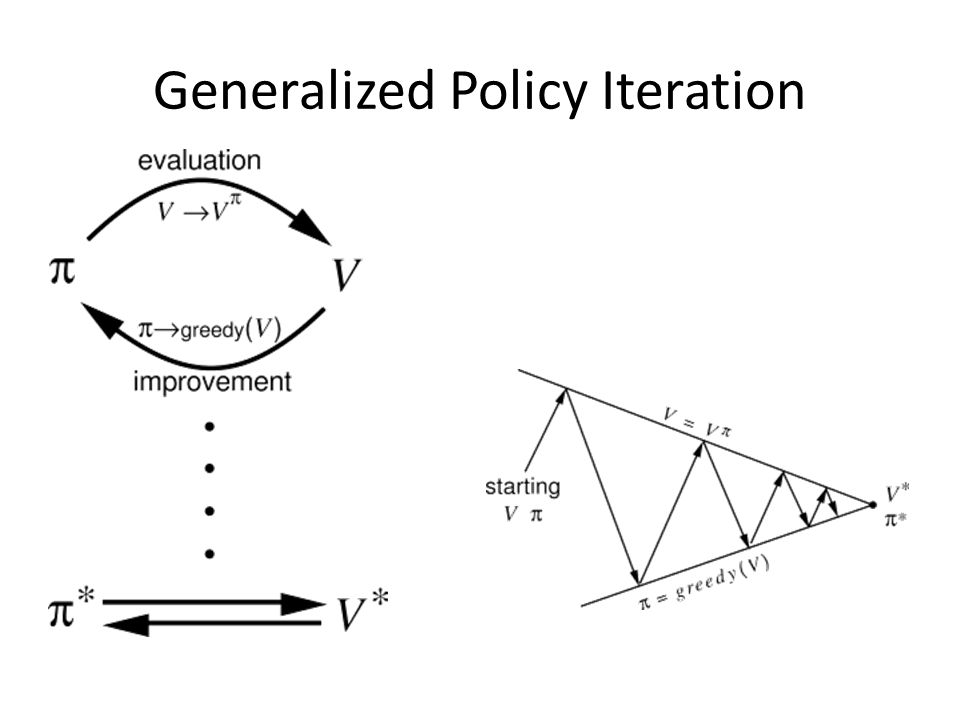
\includegraphics[width=.75\textwidth, height=.4 \textheight]{pictures/gpi_schema}
\caption{The GPI schema. (Image source: Sec. 4.6 Sutton and Barto (2017) \cite{bib:2018Sutton_RLBook}}
\end{figure}

The first process makes the value function consistent with the current policy computing the $V_\pi$.
\begin{align*}
V_{\pi}(s) =& E_\pi \left[  r + \gamma V_\pi(s^{'}) | S_t = s \right]
\end{align*}
The second process use the current value function to greedily  improve the policy:
\begin{align*}
Q_\pi(s,a) =& E\left[ R_{t+1} + \gamma V_\pi(S_{t+1}) | S_t = s, A_t = a \right]
\end{align*}
As said before, the GPI algorithm iterate over these two processes until it reaches convergence.
\begin{equation*}
\pi_0 \xrightarrow[]{\text{evaluation}} V_{\pi_0} \xrightarrow[]{\text{improve}}
\pi_1 \xrightarrow[]{\text{evaluation}} V_{\pi_1} \xrightarrow[]{\text{improve}}
\pi_2 \xrightarrow[]{\text{evaluation}} \dots \xrightarrow[]{\text{improve}}
\pi_* \xrightarrow[]{\text{evaluation}} V_*
\end{equation*}
\section{Taxonomy of Reinforcement Learning Algorithms}
\label{taxonomy}
Since the dynamics of the environment is not know, it is impossible to calculate directly the value or q-value function. 
For this reason there are two methods to approximate them, that are called \textbf{Monte Carlo Methods} (MC) and \textbf{Temporal Difference Methods} (TD).

Monte Carlo methods are based on the idea of repeated random sampling to estimate a distribution function. 
In this context, the function to approximate is the value functions need to the GPI schema explained in previous section.
In order to compute the policy evaluation step, the agent performs several rollouts of the current policy accumulating the reward and the visited states of the entire episodes. 

To accomplish the policy evaluation phase, the agent interacts with the environment accumulating experience.
Every time it visits a state, it takes note of the number of times it encounters that state ($N_ {(n)}$) and the cumulative reward obtained in that episode from that state to the end ($C_ {(n)}$).
\begin{align*}
N_{(s)} &\leftarrow N_{(s)}+1 \\
C_{(s)} &\leftarrow C_{(s)} + G_t
\end{align*}
Now having the number of times the agent has visited a state and the cumulative total reward, it is possible to approximate the value function for each state by calculating the mean return.
\begin{equation*}
V_{(s)} \leftarrow C_{(s)}/N_{(s)}
\end{equation*}
In the policy improvement step the agent chooses the action greedily with respect to the value function.
\begin{equation*}
\pi^{'}(s) = \underset{a\in A} 	\max Q(s,a)
\end{equation*}
These two steps are iteratively repeated, and it can be shown that using the law of large numbers, it is possible to prove that the algorithm converges to the optimal policy and the optimal value function.
\begin{equation*}
V_{(s)} \rightarrow v_\pi(s) \, as \, N(s) \rightarrow \infty
\end{equation*}
The problem with the Monte Carlo method is that it requires to finish the entire episode before to update the value function.

\textbf{Temporal Difference (TD)} methods are also based on the idea of GPI but differ from MC methods in the Policy Evaluation phase.
Instead of getting to the end of the episode, these methods update the value function step by step.
These methods use the current temporal estimates of the state value function, rather than relying on the complete return as the MC methods. 
This approach is called \textbf{bootstrapping}.
To obtain a better approximation the algorithm recalculate the value of every state it visits and it adds to it the reward occured in that transiction, forming the so called \textbf{TD target}.
The TD target is a slightly better approximation of the state value for that state, so the approximation must move in that direction.
To move the approximation it's necessary to calculate di difference between the old estimation and the new one, producing the \textbf{TD error}.
The entity of the update is controlled by a hyperparameter called learning rate $\alpha.$
So, this processes is repeated at each time step, and the value function is continually update.
This is called \textbf{online update}.
The formula for the value function is:
\begin{equation*}
V(S_t) \leftarrow V(S_t) + \alpha(R_{t+1} + \gamma V(S_{t+1}) - V(S_t))
\end{equation*}
The formula for the q-value function is:
\begin{equation}
\label{q-update}
Q(S_t,A_t) \leftarrow Q(S_t,A_t) + \alpha(R_{t+1} + \gamma Q(S_{t+1},A_{t+1}) - Q(S_t,A_t))
\end{equation}
These methods are referred to as \textbf{Tabular Methods} because the temporal results are cached in a table. 

The most famous algorithm in this category is \textbf{Q-learning}.  \cite{watkins1992q}.
The formula used in this algorithm to update the Q-value estimate is the equation  \ref{q_star}  that we already presented before:
\begin{align*}
q_*(s,a) =&  E\left[ R_{t+1} + \gamma  \underset{a^{'}}{\max} \, q_*\left (S_{t+1}, a^{'} \right) | S_t = s, A_t = a   \right] \\
\end{align*}
For the online update version of this formula the expectation is removed, so the formula became:
\begin{align*}
Q(s,a) =& R(s,a) + \gamma  \left(  \underset{a'}{\max}Q (s',a') \right) 
\end{align*}
Applying this TD target to the generic version of the TD formula:
\begin{align*}
Q(S_t, A_t) &\leftarrow Q(S_t, A_t) + \alpha (R_{t+1} + \gamma \max_{a \in \mathcal{A}} Q(S_{t+1}, a) - Q(S_t, A_t)) \\
\end{align*}



The formula \ref{q-update} the Q-learning formula add a $max$ operation, this simplifies the algorithm approximating the optimal action-value function, $q_*$, directly.


    \begin{algorithm}[H]
        \begin{algorithmic}
          \State Initialize $Q(s, a),$ $ \forall s \in \mathcal{S}, a \in \mathcal{A}(s),$ arbitrarily, and $Q($terminal-state$, \cdot)=0$
          \State Repeat (for each episode):
          \\\tab{Initialize $\mathcal{S}$}
          \\\tab{Repeat (for each step of episode):}
		  \\\Doubletab{ Choose $\mathcal{A}$ from $\mathcal{S}$ using policy derived from $\mathbf{Q}$ (e.g., $\epsilon-greedy$)}
          \\\Doubletab{Take Action $\mathcal{A}$, observe $\mathcal{R}$, $\mathcal{S'}$}
          \\\Doubletab{ $Q(S, A) \leftarrow Q(S, A)+\alpha\left[R+\gamma \max _{a} Q\left(S^{\prime}, a\right)-Q(S, A)\right]$}
          \\\Doubletab{ $\mathcal{S} \leftarrow \mathcal{S'}$}
          \\\tab{until $\mathcal{S}$ is terminal}
        \end{algorithmic}
    \caption{Q-learning (off-policy TD control) for estimating $\pi \approx \pi_{*}$}
    \label{alg:q-learning}
    \end{algorithm}


Both the MC and TD methods are also \textbf{Model-Free algorithms} because they solve the MDP, calculating the value or q-value function, without knowing the environment dynamics. 

However, an agent could also learn the transition probability function and the reward function and use them to accelerate the learning process or build a long term plan before acting. 
In that case, we talk about the \textbf{Model-Based algorithms} in which the model is learned, not given.

Another classification is based on how the methods find the best action to take.
The option are \textbf{Value function based} or \textbf{Policy function based}.
All the methods presented so far are value based: these methods learn the value function and then use it to choose the action with the best result.
The policy function based, instead, search directly in the policy parameters space and ends up with the best policy.

Finally there is the \textbf{Actor-Critic} method that build both the value and the policy functions.

This method is composed by two element: the actor and the critic.
The Actor is the Policy function and decides which action to take and the Critic is the Value function approximation and tells the actor how good its choice was and how to adjust it.



The critic updates value function parameters and the Actor update policy parameter using the value function suggested by the critic. 

\begin{figure}[h]
\centering
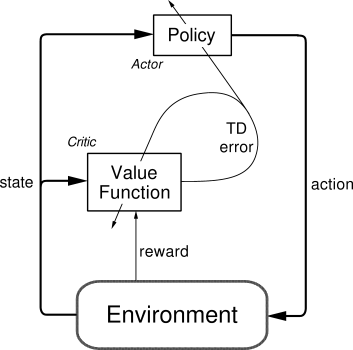
\includegraphics[width=.9 \textwidth, height=.6\textheight]{pictures/ac_schema}
\caption{ The actor-critic architecture. [Image source: Sec. 6.6 Sutton and Barto (2017)  \cite{bib:2018Sutton_RLBook}]}
\end{figure}
In the next chapter, we will introduce an actor-critic method called DDPG that will be use it to do the experiments. In chapter \ref{Chapter6}, we compare the results obtained with DDPG and the results obtained with a model-based algorithm called PlaNet.  
